\chapter{Τοπολογία Συστήματος}
\label{ch:System Topology}
Η δημιουργία φορητού (portable) λογισμικού, δηλαδή λογισμικού το οποίο μπορεί να χρησιμοποιηθεί σε συστήματα διαφορετικά μεταξύ τους, είναι δυνατή με τη χρήση αφαιρέσεων (abstractions) για το υποκείμενο σύστημα. Οι αφαιρέσεις αυτές αποκρύπτουν λεπτομέρειες της οργάνωσης του υλικού του εκάστοτε συστήματος, με την έννοια ότι από τη σκοπιά του προγραμματιστή δεν θα πρέπει να μας ενδιαφέρουν ζητήματα χαμηλού επιπέδου όπως για παράδειγμα η οργάνωση της μνήμης από φυσική άποψη (κοινόχρηστη ή κατανεμημένη) που αναφέραμε στην Υποενότητα \ref{ssec:Classification based on memory organization}, αλλά το τι εικόνα έχουμε για αυτή.

Η αφαιρετική όμως εικόνα που έχει ο προγραμματιστής για το σύστημα που καλείται να προγραμματίσει δεν του επιτρέπει να εκμεταλλευτεί στο μέγιστο τις δυνατότητές του και άρα να επιτύχει την καλύτερη δυνατή επίδοση. Για παράδειγμα, σε ένα σύστημα δύο κόμβων με κατανεμημένη φυσική οργάνωση μνήμης που όμως παρέχει κοινόχρηστο χώρο διευθύνσεων, ναι μεν ο ένας κόμβος μπορεί να προσβεί οποιαδήποτε θέση μνήμης στον άλλο κόμβο, παρόλα αυτά το κόστος της απομακρυσμένης πρόσβασης θα είναι πολύ μεγαλύτερο από αυτό της πρόσβασης στην τοπική μνήμη.

Στον προγραμματισμό παράλληλων συστημάτων που στόχος μας είναι η επίτευξη όσο το δυνατόν καλύτερων επιδόσεων, συχνά καταφεύγουμε στην εκμετάλλευση πληροφοριών που σχετίζονται με την τοπολογία. Για το λόγο αυτό γίνονται προσπάθειες δημιουργίας μεταφέρσιμου λογισμικού που όμως λαμβάνει υπόψην του την οργάνωση του υλικού σε χρόνο εκτέλεσης.

% Όπως αναφέραμε στην Υποενότητα \ref{ssec:Classification based on memory organization}, τα παράλληλα συστήματα μπορούν να ταξινομηθούν είτε βάσει της φυσικής οργάνωσης της μνήμης, είτε βάσει της εικόνας που έχει ο προγραμματιστής για αυτή, χωρίς όμως να υπάρχει απαραίτητα κάποια αντιστοίχιση μεταξύ των διαφορετικών τρόπων ταξινόμησης. Για παράδειγμα, ένα σύστημα με φυσικά κατανεμημένη μνήμη μπορεί να παρέχει κοινόχρηστο χώρο διευθύνσεων και άρα να προγραμματιστεί αντιστοίχως.


\section{Η εξέλιξη των βασικών στοιχείων ενός συστήματος}
Τα πιο σημαντικά στοιχεία που αποτελούν ένα υπολογιστικό σύστημα είναι αυτά που αφορούν τα υποσυστήματα επεξεργαστή και μνήμης.

Ένα απλό σειριακό σύστημα αποτελούνταν από έναν επεξεργαστή (ΚΜΕ - Κεντρική Μονάδα Επεξεργασίας, CPU - Central Processing Unit) ο οποίος περιείχε έναν επεξεργαστικό πυρήνα (ή απλώς πυρήνας, core) και επικοινωνούσε με την κύρια μνήμη μέσω ενός διαύλου. Με την εμφάνιση των πολυπύρηνων (multicore) οργανώσεων περισσότεροι του ενός πυρήνες ενσωματώθηκαν στον ίδιο επεξεργαστή, ενώ με την πάροδο του χρόνου προστέθηκε και ιεραρχία κρυφών μνημών.

Στα πλαίσια μιας άλλης αρχιτεκτονικής βελτίωσης, με μικρή αύξηση του μεγέθους του κυκλώματος, μπόρεσαν να ενσωματωθούν μέσα σε έναν πυρήνα 2 ή περισσότερα νήματα υλικού (H/W threads), ώστε να αξιοποιήθούν καλύτερα οι λειτουργικές μονάδες του επεξεργαστή, προσφέροντας με αυτό τον τρόπο τη δυνατότητα παράλληλης εκτέλεσης.

Τη σημερινή εποχή, μπορούμε να συναντήσουμε μεγάλα συστήματα που διαθέτουν πολλαπλούς επεξεργαστές, όπου κάθε επεξεργαστής είναι πολυπύρηνος, περιλαμβάνει ιεραρχία κρυφών μνημών και τοπική μνήμη, ενώ κάθε πυρήνας διαθέτει πολλαπλά H/W threads.

Στο Σχήμα \ref{fig:ideapad-topo} φαίνεται η οργάνωση ενός επεξεργαστή που διαθέτει 2 πυρήνες με 2 H/W threads και μία ιεραρχία κρυφών μνημών τριών επιπέδων (L1, L2, L3) στην οποία η κρυφή μνήμη του πρώτου επιπέδου διακρίνεται σε κρυφή μνήμη δεδομένων (L1d) και εντολών (L1i). Η οπτικοποίηση της τοπολογίας έγινε με το λογισμικό Portable Hardware Locality (hwloc) με το οποίο θα ασχοληθούμε περαιτέρω στην Υποενότητα \ref{ssec:hwloc}.

\begin{figure}[t]
	\centering
	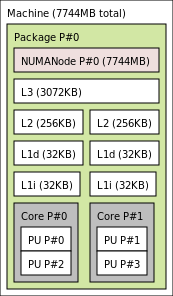
\includegraphics[width=0.25\textwidth]{Figures/ideapad-topo.png}
	\linebreak
	\caption{Η τοπολογία ενός Intel\textsuperscript{\textregistered} Core\textsuperscript{\texttrademark} i3-7100U.}
	\label{fig:ideapad-topo}
\end{figure}


\section{Συστήματα NUMA}
\label{sec:NUMA Systems}
Στην Υποενότητα \ref{ssec:Classification based on memory organization} περιγράφηκε η οργάνωση των συστημάτων ανομοιόμορφης προσπέλασης μνήμης (NUMA), τα οποία αποτελούν αρχιτεκτονική εξέλιξη των Συμμετρικών Πολυεπεξεργαστών (SMPs) που επιτρέπει την κατασκευή μεγαλύτερων παράλληλων συστημάτων.

Η πιο συχνή υλοποίηση των συστημάτων NUMA είναι ως ένα σύνολο κόμβων τύπου SMP που διαθέτουν ιεραρχία κρυφών μνημών συνδεδεμένους μεταξύ τους με ένα δίκτυο διασύνδεσης \cite{dobson2003linux}. Το δίκτυο διασύνδεσης μπορεί να είναι δακτύλιος (ring), διακοπτικό δίκτυο τύπου crossbar, από σημείο σε σημείο (point-to-point) ή πλέγμα (mesh).

Η εξασφάλιση της συνοχής των κρυφών μνημών συνήθως επιτυγχάνεται με τη χρήση ενός πρωτοκόλλου εντός του κόμβου και ενός δεύτερου πρωτοκόλλου μεταξύ των κόμβων. Όπως αναφέρθηκε νωρίτερα, ένας κόμβος SMP βασίζεται σε δίαυλο, ενώ η επικοινωνία μεταξύ των κόμβων γίνεται με πιο πολύπλοκα δίκτυα διασύνδεσης. Για το λόγο αυτό, το πρωτόκολλο συνοχής εντός του κόμβου είναι τύπου παρακολούθησης (snooping protocol), ενώ αυτό μεταξύ των κόμβων βασίζεται σε καταλόγους (directory-based protocol). Φυσικά, σε διαφορετικές οργανώσεις συστημάτων NUMA μπορούμε να συναντήσουμε και άλλες στρατηγικές επίτευξης συνοχής, όπως αυτή της μη αποθήκευσης κοινόχρηστων δεδομένων στις κρυφές μνήμες.

Όπως γίνεται γρήγορα αντιληπτό, ο προγραμματισμός αυτών των συστημάτων συνήθως απαιτεί να εστιάσουμε στην τοπικότητα, δηλαδή τη χρήση πόρων που βρίσκονται στη μικρότερη δυνατή απόσταση και την μείωση της επικοινωνίας μεταξύ των κόμβων \cite{bligh2004linux}. Για την επίτευξη της τοπικότητας και άρα τη συγγραφή πιο αποδοτικών προγραμμάτων, η εκμετάλλευση πληροφορίας που σχετίζεται με την τοπολογία είναι απαραίτητη.

% Ήδη από την έκδοση 2.5 του Linux Kernel προστέθηκε η βασική υποδομή για υποστήριξη συστημάτων NUMA, που περιλαμβάνει μεταξύ άλλων αναγνώριση της τοπολογίας, δέσμευση μνήμης και χρονοδρομολόγηση διεργασιών \cite{dobson2003linux}.

Στο Σχήμα \ref{fig:parade-topo} φαίνεται η οργάνωση του \texttt{parade}, ενός NUMA συστήματος με τέσσερις κόμβους τύπου SMP που διαθέτει η Ομάδα Παράλληλης Επεξεργασίας του Πανεπιστημίου Ιωαννίνων και η οργάνωσή του αποτελεί την πλέον συνηθισμένη.

\begin{figure}[t]
	\centering
	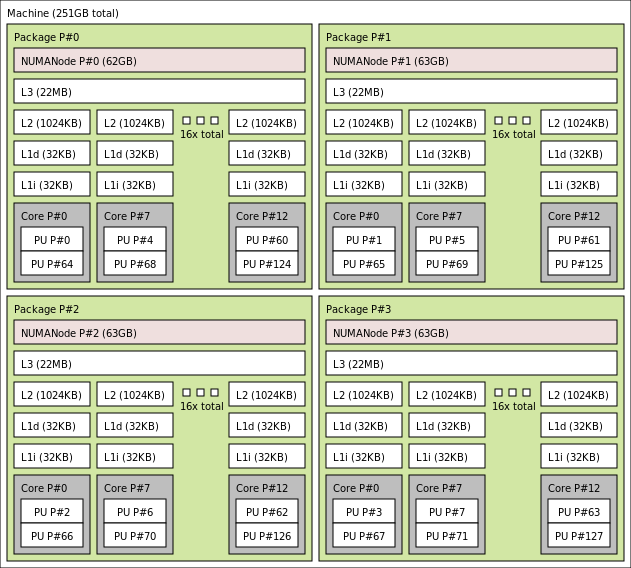
\includegraphics[width=0.8\textwidth]{Figures/parade-topo.png}
	\linebreak
	\caption{Η τοπολογία ενός Dell PowerEdge R840 με 4 Intel\textsuperscript{\textregistered} Xeon\textsuperscript{\textregistered} Gold 6130.}
	\label{fig:parade-topo}
\end{figure}


\section{Βοηθητικά Εργαλεία}
\label{sec:Utility Tools}
Για την εκμετάλλευση της τοπολογίας ενός συστήματος έχουν αναπτυχθεί διάφορα εργαλεία όπως η βιβλιοθήκη Portable Hardware Locality (hwloc) και η \texttt{libnuma}.

\subsection{hwloc}
\label{ssec:hwloc}
Η βιβλιοθήκη Portable Hardware Locality παρέχει μία φορητή αφαίρεση (abstraction) της τοπολογίας που διαθέτουν υπολογιστικά συστήματα με σύγχρονες αρχιτεκτονικές. Ο κύριος λόγος χρήσης της είναι η συγκέντρωση πληροφοριών σχετικά με πολύπλοκα παράλληλα συστήματα, με στόχο την κατάλληλη και αποδοτική εκμετάλλευσή τους \cite{broquedis2010hwloc}. 

\noindent Τα λειτουργικά συστήματα που υποστηρίζονται είναι τα εξής:
\begin{itemize}
	\item Linux
	\item Solaris, AIX, HP-UX
	\item NetBSD, FreeBSD, kFreeBSD/GNU
	\item Darwin / OS X
	\item Microsoft Windows
	\item IBM BlueGene/Q Compute Node Kernel (CNK)
\end{itemize}

\subsubsection{Τα στοιχεία που απαρτίζουν την τοπολογία}
Η hwloc μπορεί να αναγνωρίσει τα εξής στοιχεία υλικού:
\begin{itemize}
	\item Κόμβους συστημάτων NUMA (NUMA nodes)
	\item Υποδοχές επεξεργαστών (packages, πρώην sockets)
	\item Κρυφές μνήμες (caches)
	\item Πυρήνες (cores)
	\item H/W threads (PUs - Processing Units)
	\item Σύσκευές εισόδου-εξόδου όπως:
	\begin{itemize}
		\item Συσκευές PCI
		\item Επιταχυντές OpenCL, CUDA και Xeon Phi
		\item Προσαρμογείς δικτύου (network interfaces) όπως InfiniBand	
	\end{itemize}
\end{itemize}

Με την ορολογία της hwloc στη διάθεση μας, ας ανατρέξουμε στο Σχήμα \ref{fig:parade-topo} που απεικονίζεται η τοπολογία του συστήματος parade. Στο σχήμα αυτό βλέπουμε 4 επεξεργαστές ο καθένας εκ των οποίων διαθέτει 12 πυρήνες, και ιεραρχία κρυφών μνημών τριών επιπέδων (L1i \& L1d, L2, L3). Τα επίπεδα ένα και δύο των κρυφών μνημών είναι κοινά ανά πυρήνα, ενώ το επίπεδο τρία είναι κοινό για όλους τους πυρήνες του επεξεργαστή. Επίσης, κάθε πυρήνας διαθέτει δύο H/W threads τα οποία μοιράζονται τους πόρους του πυρήνα (π.χ. κρυφές μνήμες).

\subsubsection{Οι εντολές lstopo και lstopo-no-graphics}
Οι εντολές \texttt{lstopo} και \texttt{lstopo-no-graphics} συμπεριλαμβάνονται στην hwloc και χρησιμοποιούνται για την προβολή της τοπολογίας ενός συστήματος σε διαφορετικές μορφές, όπως κείμενο ASCII, SVG, PDF, Postscript, PNG, XML και αρκετές άλλες.

Τα Σχήματα \ref{fig:ideapad-topo} και \ref{fig:parade-topo} είναι αποτέλεσμα αυτών των δύο εντολών. Η αναπαράσταση του Σχήματος \ref{fig:ideapad-topo} σε μορφή κειμένου ASCII είναι η ακόλουθη\footnote{Για λόγους απλότητας έχουν παραληφθεί οι συσκευές Εισόδου/Εξόδου.}:

\begin{verbatim}
Machine (7744MB total)
  Package L#0
    NUMANode L#0 (P#0 7744MB)
    L3 L#0 (3072KB)
      L2 L#0 (256KB) + L1d L#0 (32KB) + L1i L#0 (32KB) + Core L#0
        PU L#0 (P#0)
        PU L#1 (P#2)
      L2 L#1 (256KB) + L1d L#1 (32KB) + L1i L#1 (32KB) + Core L#1
        PU L#2 (P#1)
        PU L#3 (P#3)
\end{verbatim}

Η διαφορά των δύο εντολών είναι ότι η δυνατότητα γραφικής αναπαράστασης (π.χ. PNG) υπάρχει μόνο στην πρώτη. Αυτό συμβαίνει για τη μείωση των εξαρτήσεων με τις σχετικές βιβλιοθήκες γραφικών που χρησιμοποιούνται για τη δημιουργία των οπτικοποιήσεων. Για παράδειγμα, στο σύστημα parade που χρησιμοποιείται για τη διεξαγωγή πειραματικών μετρήσεων δεν υπάρχουν οι απαραίτητες βιβλιοθήκες γραφικών. Για το λόγο αυτό χρησιμοποιήθηκε η εντολή \texttt{lstopo-no-graphics} για την αποθήκευση της τοπολογίας σε μορφή XML και σε διαφορετικό σύστημα με τις κατάλληλες βιβλιοθήκες εγκατεστημένες χρησιμοποιήθηκε η μορφή XML ως είσοδος στην εντολή \texttt{lstopo} για την παραγωγή αρχείου PNG.


\subsubsection{Η διεπαφή προγραμματισμού εφαρμογών (API)}
Η βασική διεπαφή προγραμματισμού εφαρμογών (API) της hwloc είναι διαθέσιμη μέσω του αρχείου \texttt{hwloc.h}.

Η τοπολογία του υποκείμενου συστήματος αναπαρίσταται ως μία δεντρική δομή από αντικείμενα και αποθηκεύεται σε μία μεταβλητή τύπου \texttt{hwloc\_topology\_t}. Στη ρίζα του δέντρου υπάρχει πάντα ένα αντικείμενο τύπου Machine που αναπαριστά ολόκληρο το υποκείμενο μηχάνημα/σύστημα, ενώ στα φύλλα του δέντρου υπάρχουν πάντα PUs ή αλλιώς H/W threads που αποτελούν το μικρότερο διαθέσιμο επεξεργαστικό στοιχείο. Καμία άλλη παραδοχή δεν είναι δυνατόν να γίνει για τη μορφή της τοπολογίας (π.χ. βάθος, τύποι αντικειμένων που την απαρτίζουν κλπ).

Για τη διαχείριση της μεταβλητής τύπου \texttt{hwloc\_topology\_t} χρησιμοποιούνται οι εξής βασικές συναρτήσεις των οποίων η λειτουργία είναι εύκολα κατανοητή από το όνομά τους:
\begin{itemize}
	\item \texttt{hwloc\_topology\_init()}
	\item \texttt{hwloc\_topology\_load()}
	\item \texttt{hwloc\_topology\_destroy()}
\end{itemize}

Αφού αρχικοποιηθεί και φορτωθεί η τοπολογία με τις δύο πρώτες κλήσεις, μπορεί να γίνει αναδρομική διάσχιση του δέντρου για την ανακάλυψη των διαφορετικών συστατικών του στοιχείων (packages, NUMA nodes, caches, cores, PUs). Η hwloc διαθέτει πλήθος χρήσιμων συναρτήσεων που διευκολύνουν είτε την αναδρομική διάσχιση, είτε τη διάσχιση ενός μόνο επιπέδου και επιτρέπουν:
\begin{itemize}
	\item την εύρεση του αντικειμένου στη ρίζα της τοπολογίας (\texttt{hwloc\_get\_root\_obj()}).
	\item την εύρεση του πλήθους των αντικειμένων που έχουν συγκεκριμένο τύπο ή βάθος (\texttt{hwloc\_get\_nbobjs\_by\_type()} και \texttt{hwloc\_get\_nbobjs\_by\_depth()}).
	\item την εύρεση αντικειμένων με συγκεκριμένο τύπο ή σε συγκεκριμένο βάθος (\texttt{hwloc\_get\_obj\_by\_type()} και \texttt{hwloc\_get\_obj\_by\_depth()}).
	\item την εύρεση του επόμενου στη σειρά αντικειμένου με συγκεκριμένο τύπο ή βάθος (\texttt{hwloc\_get\_next\_obj\_by\_type()} και \texttt{hwloc\_get\_next\_obj\_by\_depth()}).
\end{itemize}


\subsubsection{Άλλες δυνατότητες της hwloc}
Πέρα από τη συγκέντρωση πληροφοριών που σχετίζονται με την τοπολογία του υποκείμενου συστήματος, η hwloc μπορεί να χρησιμοποιηθεί για την ανάθεση νημάτων (thread binding) σε επεξεργαστές, τη διαχείριση μνήμης με δυνατότητα δέσμευσης τμημάτων μνήμης (memory binding) σε συγκεκριμένους κόμβους NUMA. Παρόλα αυτά, η χρήση των διαθέσιμων λειτουργιών υπόκειται στις δυνατότητες του εκάστοτε λειτουργικού συστήματος.


\subsection{libnuma}



\section{Χρήση τοπολογίας στο OpenMP}
\label{sec:Topology in OpenMP}
Η διπλωματική εργασία περιέχει $\nu$ κεφάλαια.
